\begin{figure}[H]
    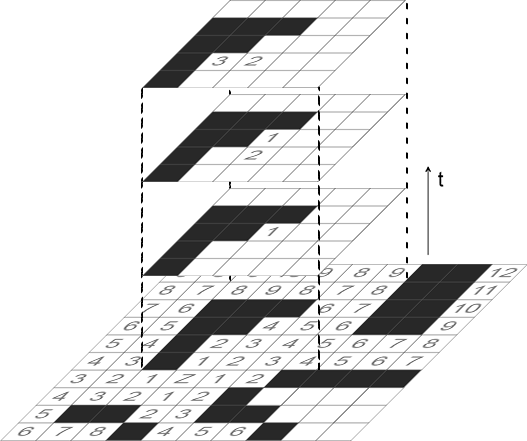
\includegraphics[width=9cm]{images/distance_localmap.png}
    \centering
    \caption{Entfernungs- und Umgebungskarte}
    \label{fig:distance_localmap}
\end{figure}
Die Umgebungskarte bildet einen Ausschnitt aus der Entfernungskarte dar. Im Gegensatz zur Entfernungskarte besitzt die Umgebungskarte eine Zeitdimension (siehe Abbildung \ref{fig:distance_localmap}). Damit ist es möglich dynamische Objekte, also andere Agenten, in die Wegplanung mit einzubeziehen. Dies beschreibt auch die Hauptfunktion dieser Karte. In die Umgebungskarte werden die, über Nachrichten von den anderen Agenten übermittelten, geplanten Wege eingetragen und für die eigene Wegplanung bereitgestellt. Die Dimensionen der Umgebungskarte sind immer ungerade, da die mittlere Zelle die aktuelle Position des Agenten spiegelt. Die Zeitdimension \(t\) zeigt von dem aktuellen Zeitpunkt aus in die Zukunft, wird aber durch die zeitlichen Berechnungstiefe \(t\textsubscript{max}\) begrenzt. Abbildung \ref{fig:distance_localmap} zeigt, dass die statischen Hindernisse von der Entfernungskarte übernommen werden, die Entfernungen jedoch nicht. Die Zellen halten andere Daten. Eine Zelle der Umgebungskarte ist entweder frei, von einen statischen Hindernis belegt oder von einem anderen Agenten reserviert. \cite{book:regele}